\chapter{Estimation Theory}
\label{ch:estimation-theory}

\section{Estimators: the interface between sampling and guarantees}

Database systems rarely compute quantities exactly: sketches compress frequency vectors, samplers select a few rows or a few random spanning trees, and privacy mechanisms deliberately add noise. Estimation theory is what lets a paper say something rigorous about the resulting number. Whenever a data structure or mechanism reports a value $\hat\theta$ together with a claim of the form ``within $\varepsilon$ of the truth with probability at least $1-\delta$,'' an \emph{estimator} has been constructed and its error has been bounded. The three classical questions transfer verbatim: is $\hat\theta$ \emph{unbiased}, how large are its \emph{variance} or mean-squared error, and can \emph{any} estimator in the same situation do better, i.e., what does a \emph{minimax} or information-theoretic lower bound permit \cite{estimation-theory-bg1,estimation-theory-bg2}? In the SIGMOD'26 corpus, estimation theory is used by 27 of the 228 tagged papers and is the most frequent companion of the \emph{error-bound} (16 papers) and \emph{probabilistic-guarantee} (13 papers) tags: it is the tool that turns a data reduction into a guarantee.

The workflow typically runs backwards from the target guarantee: build a sketch or sampler; read an estimator off it; bound the estimator's variance; convert variance into a confidence statement with a concentration inequality; pay a union bound over the keys, nodes, or rounds that must be simultaneously correct; and, in the strongest papers, prove a matching lower bound showing the error or the space is optimal.

\section{The tool}

\paragraph{Bias--variance decomposition.} For an estimator $\hat\theta$ of a parameter $\theta$,
\begin{equation}
\mathrm{MSE}_\theta(\hat\theta)
= \mathbb{E}\big[(\hat\theta-\theta)^2\big]
= \underbrace{\big(\mathbb{E}[\hat\theta]-\theta\big)^2}_{\text{squared bias}}
+ \underbrace{\mathrm{Var}(\hat\theta)}_{\text{variance}},
\label{eq:bias-variance}
\end{equation}
and every design decision in a sketch or mechanism is a move between the two terms. Unbiasedness ($\mathbb{E}[\hat\theta]=\theta$) is prized because variances \emph{add} over independent contributions --- per-key counters, per-round messages, per-node estimates --- so one variance computation feeds Chebyshev or Chernoff bounds and yields the $(\varepsilon,\delta)$ statement directly \cite{estimation-theory-bg3}. Its fragility matters equally: unbiasedness is destroyed by nonlinear post-processing, $\mathbb{E}[g(X)] \neq g(\mathbb{E}[X])$, so estimating $x^p$ from an unbiased estimate of $x$ requires a Taylor-series or geometric-mean correction rather than plugging in.

\paragraph{Unbiasedness versus minimax.} A single unbiased estimator says nothing about optimality. The minimax risk
\[
\inf_{\hat\theta}\;\sup_{\theta\in\Theta}\;\mathbb{E}\big[(\hat\theta-\theta)^2\big]
\]
benchmarks \emph{all} estimators at once. For unbiased estimators the Cram\'er--Rao inequality $\mathrm{Var}_\theta(\hat\theta)\ge 1/I(\theta)$, with $I(\theta)=\mathbb{E}\big[(\partial_\theta\log p_\theta(X))^2\big]$ the Fisher information, gives a local benchmark; two-point (Le Cam) and Fano arguments give distribution-free ones \cite{estimation-theory-bg2}. In DB papers the ``information'' is usually combinatorial rather than Fisherian: the sensitivity of a query under neighboring inputs, the norm of the stream, or the entropy of any encoding of the sketch. The last turns estimation error into a space lower bound: if the estimator must be $(E,\delta)$-accurate, the sketch state must be incompressible below the entropy of what it has to distinguish \cite{estimation-theory-bg1}.

\paragraph{The estimator-to-bound pipeline.} Corpus papers instantiate the same five-step pipeline:
(i) construct $\hat\theta$ from a sketch, a sample, or a randomized mechanism, and check its expectation;
(ii) bound $\mathrm{Var}(\hat\theta)$ or a sub-Gaussian proxy in terms of structural parameters (stream norms, degrees, sensitivities);
(iii) apply a concentration inequality to pass from variance to a per-quantity $(\varepsilon,\delta)$ statement;
(iv) union-bound over all coordinates that must hold simultaneously, paying a $\log(\#\text{quantities})$ factor;
(v) match with a lower bound (variance, Le~Cam/Fano, or entropy) to certify optimality \cite{estimation-theory-bg2,estimation-theory-bg3,estimation-theory-bg4}.

\begin{center}
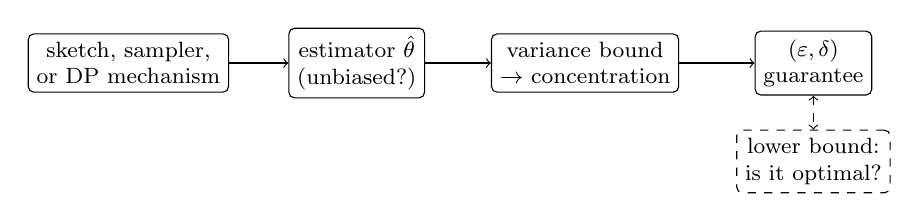
\begin{tikzpicture}[
  box/.style={draw, rounded corners=2pt, inner sep=3pt, align=center, font=\footnotesize}]
\node[box] (s)   at (0,0)    {sketch, sampler,\\ or DP mechanism};
\node[box] (e)   at (2.9,0)  {estimator $\hat\theta$\\ (unbiased?)};
\node[box] (v)   at (5.8,0)  {variance bound\\ $\to$ concentration};
\node[box] (g)   at (8.7,0)  {$(\varepsilon,\delta)$\\ guarantee};
\node[box, dashed] (lb) at (8.7,-1.25) {lower bound:\\ is it optimal?};
\draw[->] (s) -- (e);
\draw[->] (e) -- (v);
\draw[->] (v) -- (g);
\draw[<->, dashed] (g) -- (lb);
\end{tikzpicture}

\smallskip
{\small The estimator pipeline: every exemplar below walks left to right; the strongest also close the loop.}
\end{center}

\section{Exemplars from the SIGMOD'26 corpus}

\subsection{Perfect $\ell_p$ sampling from exponential variables (streaming)}

One-pass streaming algorithms must output a single index $i$ distributed with probability proportional to $|f_j|^p$, the ideal $\ell_p$ sample; the classical difficulty is that the stream must be tracked under this unusual distribution. The paper treats the output index itself as the estimator and bounds its accuracy per coordinate.

\begin{theorem}[Theorem 1 of \cite{sigmod26-247}: $\ell_p$ sampler]
For any constant $p\in(0,2]$, there is a one-pass streaming algorithm that runs in space $\widetilde{O}(\log^{c(p)} n\cdot\log(1/\delta))$ and outputs an index $i$ such that, with probability at least $1-\delta$, for every $j\in[n]$,
\[
\Pr[i=j] \;=\; \frac{|f_j|^p}{\lVert f\rVert_p^p} \;\pm\; \frac{1}{\mathrm{poly}(n)},
\qquad
c(p)=\begin{cases} 1 & 0<p<2,\\ 2 & p=2.\end{cases}
\]
\end{theorem}

\begin{corollary}[Corollary 3.3 of \cite{sigmod26-247}]
Let $f\in\mathbb{R}^n$ be a frequency vector and let $(e_1,\dots,e_n)$ be i.i.d.\ exponential random variables with rate $1$. Define $z_i = f_i/e_i^{1/p}$ and let $(D^{(1)},\dots,D^{(n)})$ be the anti-rank vector of the vector $(z_1^{-p},\dots,z_n^{-p})$. Then
\[
\Pr\big[D^{(1)}=i\big] \;=\; \frac{|f_i|^p}{\lVert f\rVert_p^p}.
\]
\end{corollary}

What is estimated is a whole distribution rather than a scalar, and the error bound is an $\ell_\infty$ bound on the sampled probabilities. The estimator trick is the exponential race: by scaling, $e_i/f_i^p = z_i^{-p}$ is exponential with rate $|f_i|^p$, so the minimum is attained at $i$ with exactly $\ell_p$ probability; the streaming algorithm then only has to track the rescaled vector $z$ (via BPTree, CountSketch, and AMS sketches), repairing the nonlinear $x^p$ step with Taylor-series and geometric-mean estimators, with Chebyshev and union bounds supplying the $\pm 1/\mathrm{poly}(n)$ accuracy. \cite{sigmod26-247}\pods

\subsection{Unbiased Laplace-noised walk counting (local differential privacy on graphs)}

Counting $k$-line walks in a graph where every node privatizes its own view (edge-local DP) forces fresh Laplace noise at each of $k$ synchronous rounds, so the naive error compounds with $k$; the question is how much accuracy a $k$-round message-passing mechanism can retain.

\begin{theorem}[Theorem 4.2 of \cite{sigmod26-012}]
For any graph $G$, walk length $k$, and parameters $\varepsilon$ and $\beta$, the $k$-round mechanism $\mathcal{M}_{k\text{-wk}}$ satisfies $\mathbb{E}[\mathcal{M}_{k\text{-wk}}(G,\varepsilon)] = W_k$, and with probability at least $1-\beta$,
\[
\big|\mathcal{M}_{k\text{-wk}}(G,\varepsilon) - W_k\big|
\;\le\; k\gamma\sqrt{N}\,\big(d(G)+\gamma\big)^{k-1}
\;=\; \widetilde{O}\big(\sqrt{N\, d(G)^{k-1}}\big),
\]
where $\gamma = 2k\sqrt{8\log(2kN/\beta)}/\varepsilon = \widetilde{O}(1)$, with $N$ the number of nodes and $d(G)$ a degree parameter of $G$.
\end{theorem}

What is estimated is $W_k$, the number of $k$-line walks; the bound is unbiasedness plus a high-probability additive error of $\widetilde{O}\big(\sqrt{N\,d(G)^{k-1}}\big)$, improving on the typical $O(N^{k/2})$ of naive Laplace counting. The estimator trick is sensitivity control by induction: each round adds per-node Laplace noise scaled by the running maximum $\lVert X^{(\ell-1)}\rVert_\infty$, a Laplace concentration bound (failure budget $\beta'/N$ per node per round) yields $\lVert X^{(\ell)}\rVert_\infty \le (d(G)+\gamma)^{\ell}$, and union bounds close the loop; a complementary variance lower bound of $\Omega(N^{k+1})$ for the baseline estimator, obtained by summing variances over all oriented $k$-line walks, shows the multi-round design is genuinely needed. \cite{sigmod26-012}

\subsection{Variance recursion and an entropy lower bound for expandable sketches}

A frequency-estimation (FE) sketch for streams of unknown, unbounded length must expand as the stream grows; the paper asks both how accurate such a sketch can be and how much memory the expansion forces, matching the two sides.

\begin{lemma}[Variance of the sketch \cite{sigmod26-231}]
Like CountSketch, the sketch provides unbiased estimates. Moreover, letting $V(F)$ denote its estimation variance when using a size function $W(\cdot)$ and one array on a stream with squared $\ell_2$-norm $F=\sum_y (f(y))^2$, we have at the end of epoch $i$ that
\[
V(F_{i+1}) \;\le\; \frac{1}{W_i}\cdot\sum_{j=0}^{i} 2^{\,i-j}\cdot\big(F_{j+1}-F_j\big),
\]
where $F_j$ denotes the squared $\ell_2$-norm of the stream at the start of epoch $j$.
\end{lemma}

\begin{theorem}[Space lower bound \cite{sigmod26-231}]
Consider an FE sketch with only overestimation errors that processes growing streams with an error bound of $E(N)$ and a confidence of $1-\delta$. Such a sketch must use at least
\[
\frac{N}{E(N)}\cdot\Big[\Omega\Big(\log\tfrac{1}{\delta}+\log\log\tfrac{N}{E(N)}\Big)-\Theta(1)\Big]
\]
bits of memory at some point in time while processing a stream.
\end{theorem}

What is estimated are per-key frequencies, unbiasedly as in CountSketch; the error bound is a variance recursion over geometrically spaced epochs, each past expansion contributing with weight $2^{\,i-j}$, and Markov/Chebyshev convert it into the stated confidence. The complementary trick is the lower bound: an entropy-incompressibility argument (by reduction to filters) shows any sketch achieving error $E(N)$ at confidence $1-\delta$ must pay the displayed bits, and the constructed sketch lands within a small logarithmic factor of it --- the estimation-theoretic ideal of a matched pair. \cite{sigmod26-231}

\subsection{Concentration-chosen sample sizes for influence minimization}

Blocking nodes to curb time-critical misinformation spread requires maximizing a benefit function $D(\cdot)$ that is $\#P$-hard to evaluate and non-submodular, so greedy must run on sampled surrogates; the question is how many samples suffice for the greedy choice to provably transfer to the true objective.

\begin{theorem}[Theorem 6.7 of \cite{sigmod26-373}]
Given $0\le\varepsilon,\delta\le 1$, CBFM returns $B^{*}$ satisfying
\[
\Pr\big[D(B^{*}) \;\ge\; \tau\big(1-\tfrac{1}{e}-\varepsilon\big)\cdot D(B_{o})\big] \;\ge\; 1-3\delta,
\]
where $B_{o}$ denotes an optimal solution.
\end{theorem}

What is estimated is $D(B)$ itself, by an unbiased estimator $\hat D(B)$ built from reverse-score sample sets (GRS/TRS) whose coverage terms are unbiased; the error bound is an end-to-end $(1-1/e-\varepsilon)$-style approximation holding with probability $1-3\delta$, where $\tau$ reflects that greedy optimizes $D$ through the submodular surrogates sandwiching it ($D_L \le D \le D_{U'}$). The estimator trick is to derive the sample threshold analytically: concentration bounds fix the maximal sample size $\theta_{\max}$, and three union-bound events account for the $3\delta$. \cite{sigmod26-373}

\subsection{How many random trees? (biharmonic distance)}

Pairwise biharmonic distance requires quantities from the square of the Laplacian pseudoinverse, which no near-linear graph algorithm computes exactly; the paper reformulates the distance and estimates each term by averaging over randomly sampled spanning trees.

\begin{theorem}[Theorem 6.3 of \cite{sigmod26-102}]
If $\omega_t = d_v^2\Delta^2\log(2n/\delta)/(2\varepsilon^2)$, FastTree samples $\omega_t$ trees, and the corresponding estimators satisfy that for each node $u$,
\[
\big|x_a(u)-\tilde{x}_a(u)\big| \le \varepsilon
\qquad\text{and}\qquad
\big|x_b(u)-\tilde{x}_b(u)\big| \le \varepsilon .
\]
\end{theorem}

What is estimated are the two terms $x_a,x_b$ of the reformulated distance (a pivoted identity rewrites $\beta(s,t)$ via $\widehat L_v^{-1}$ and a rank-structured correction), each by the average of $\omega_t$ unbiased tree-sampling estimators grounded in electrical-network/Kirchhoff identities; the error bound is per-node $\varepsilon$-accuracy from Chernoff--Hoeffding plus a union bound over all $n$ nodes. The trick is visible in the sample count itself: it is exactly the canonical Hoeffding size (range scale $d_v\Delta$, with $d_v$ the pivot degree and $\Delta$ a graph parameter) squared, times $\log(2n/\delta)$, over $2\varepsilon^2$ --- the matrix inverse is replaced by an expectation over absorbing random walks. \cite{sigmod26-102}

\begin{reachbox}{When to reach for estimation theory}
\begin{itemize}
\item You report a number derived from a sketch, a sample, or a randomized mechanism, and must attach error bars or an $(\varepsilon,\delta)$ confidence to it.
\item Unbiasedness is the workhorse: it makes variances add across keys, rounds, or nodes, so one variance bound plus Chebyshev/Chernoff delivers the guarantee.
\item Nonlinearity breaks unbiasedness ($\mathbb{E}[g(X)] \neq g(\mathbb{E}[X])$); fix it with Taylor-series or geometric-mean corrections instead of ignoring the bias.
\item To size a structure, invert the concentration bound: sample counts of the form $\omega \approx \mathrm{range}^2\log(n/\delta)/(2\varepsilon^2)$ should fall out analytically, not be tuned.
\item To certify optimality, pair the upper bound with a variance, Cram\'er--Rao, Le~Cam/Fano, or entropy-incompressibility lower bound; matching within logarithmic factors is the gold standard.
\item Remember the two hidden costs: union bounds charge $\log(\#\text{quantities})$, and minimax bounds rate the estimator class, not your implementation.
\end{itemize}
\end{reachbox}
